\section{Introduction}
\label{sec:introduction}

Reinforcement learning with verifiable rewards (RLVR) has emerged as an effective
approach for improving language-model reasoning, particularly in mathematical and
programmatic domains where solutions can be evaluated with inexpensive, objective
feedback~\citep{shao2024deepseekmath,guo2025deepseek}. Extending this paradigm to
vision-language models requires training data whose questions are grounded in
visual content, whose answers can be verified exactly, and whose variation extends
beyond a narrow set of templates. Recent multimodal RL methods report gains in
visual mathematics, counting, spatial reasoning, and general visual
understanding~\citep{liu2025visualrft,huang2025visionr1,peng2025lmmr1,
meng2025mmeureka}, yet constructing visual training data that support broad and
transferable reasoning remains a central bottleneck.

Existing work has pursued two main strategies. Large training mixtures broaden
coverage by combining many datasets with task-specific rewards
~\citep{sarch2026vero}, but they inherit heterogeneous task granularity, sampling
units, and reasoning boundaries from their source collections. Procedural systems
instead provide exact supervision and controlled generation, but typically focus
on a single scene grammar or a small set of closely related objectives, such as
jigsaws, visual logic puzzles, games, or abstract perception tasks
~\citep{wang2025jigsawr1,feng2025visualsphinx,tong2025gamerl,
alam2026sphinx,yang2026tron}. As a result, breadth, controllability, and exact
verification are rarely combined within one coherent task organization.

We introduce \trace, a taxonomy-guided environment that addresses this gap by
separating visual construction from reasoning computation. A scene grammar defines
the objects, relations, and layout family that can be rendered; a task program
specifies the computation and answer type; and a reward contract defines exact
verification. Bounded query variation changes a meaningful task argument, such as
extremum direction, without creating a separate task. Building on structured scene
representations and executable question programs in CLEVR and Task Me Anything
~\citep{johnson2017clevr,zhang2024taskmeanything}, \trace uses this decomposition
not only to generate instances, but also to define the units used for sampling,
verification, and cross-domain analysis.

This organization yields 1,000 tasks over 277 scene grammars spanning 11 visual
domains. Each instance is generated from a semantic state on which the task program
is executed; the same state determines the image, prompt, typed answer, and verifier
state. Supervision therefore follows directly from the task computation rather than
from labels assigned after rendering. The environment supports controlled variation
in both semantic content and visual realization while preserving stable task
identity and exact rewards. Figure~\ref{fig:domain-montage} illustrates the resulting
visual breadth.

\begin{figure}[t]
  \centering
  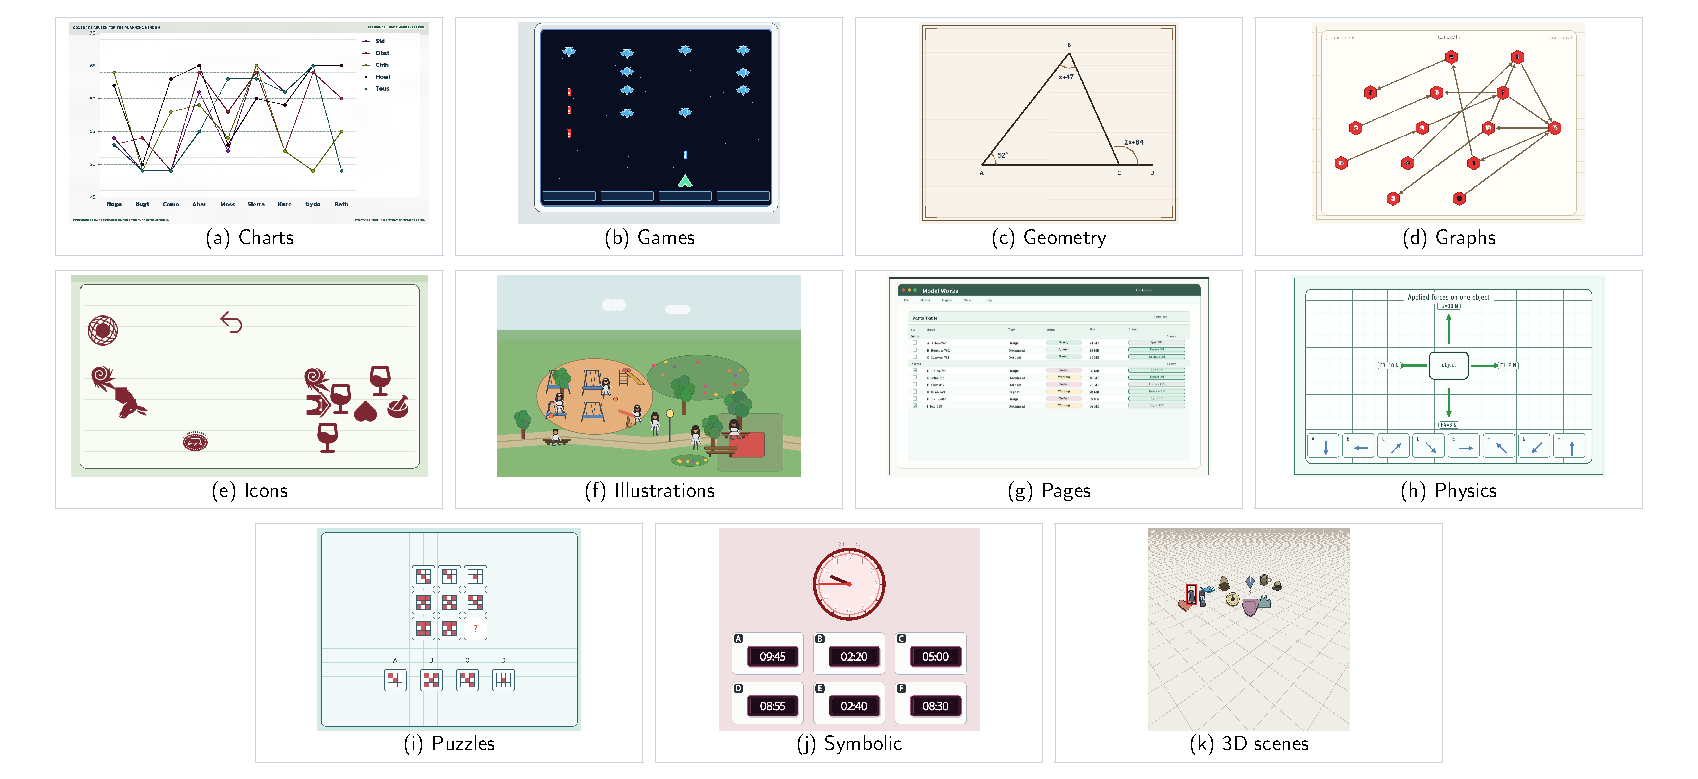
\includegraphics[width=\textwidth]{figures/domain_montage.pdf}
  \caption{Representative instances from the 11 visual domains in \trace,
  spanning charts, games, geometry, graphs, icons, illustrations, pages,
  physics, puzzles, symbolic notation, and three-dimensional scenes.}
  \label{fig:domain-montage}
\end{figure}

We use \trace to test whether RLVR on procedural visual tasks transfers beyond
held-out instances from the same environment. Qwen2.5-VL-3B and
Qwen2.5-VL-7B are trained on the same 64,000 \trace instances and evaluated on
24 external visual-reasoning benchmarks. Training improves the benchmark
macro-average by 3.51 percentage points at 3B and 4.06 points at 7B, providing
evidence that broad procedural training can support transfer beyond the
generated task distributions.

Our contributions are:
\begin{itemize}
    \item A program-centered taxonomy that separates scene grammars, executable
    task programs, and bounded query variation, providing stable task units across
    1,000 tasks, 277 scene grammars, and 11 visual domains;

    \item An executable generator--renderer--verifier environment in which images,
    prompts, typed answers, verifier states, and replayable instance traces derive
    from shared semantic state, enabling exact supervision and controlled semantic
    and visual variation; and

    \item A two-scale RLVR study showing gains of 3.51 and 4.06 points on the
    24-benchmark macro-average at 3B and 7B, respectively, with positive mean
    changes on 21 of 24 benchmarks at 3B and all 24 benchmarks at 7B.
\end{itemize}